%Edit 019 ZZZ to call document number nnnn 
%Edit FM-WP4 Code structure and coordination YYWP to Workpackage description
%Edit 3.2 YYACT to Activity number(s)
%Edit Investigate DSL and code generation techniques YYTITLE to bid title - Words Start with Caps
\documentclass[11pt,twoside,a4paper]{article}
%%======================================================================
%% PACKAGES:
%%
%\usepackage{times}               % Times+Helvetica+Courier fonts
\usepackage{helvet}              % helvetica + cmr
\usepackage{fancyhdr}       % package for headers/footers
\usepackage{amsmath}
\usepackage{amssymb}
\usepackage{graphicx}            % Graphics.
%\usepackage{a4}                  % page layout to fit A4
%\usepackage{lastpage}            % get page no of last page
%\usepackage{ifthen}              % logical branching
\usepackage{hyperref}            %insert hyper-links
\usepackage{latexsym}
% uncomment the following to override auto page total
%\pptotal{20}
%%======================================================================

% ensure sans-serif font used throughout
\renewcommand{\familydefault}{\sfdefault}

\newcommand{\culhamissueno}{1.00}%<==edit
\newcommand{\culhamshorttitle}{CD/EXCALIBUR-FMS/019}%<==edit
\newcommand{\Sec}[1]{Section~\ref{sec:#1}}
\newcommand{\Fig}[1]{Figure~\ref{fig:#1}}
\newcommand{\Eq}[1]{Equation~(\ref{eq:#1})}
\newcommand{\Eqs}[2]{Equations(\ref{eq:#1}) and~(\ref{eq:#2})}
\newcommand{\Figs}[2]{Figures~\ref{fig:#1}--~\ref{fig:#2}}
%Bold lc for script names, tt for computer code and file-names
%\F{NEPTUNE} always in caps
\newcommand{\F}[1]{\textsc{#1}}
\newcommand{\B}[1]{\textbf{#1}}
\newcommand{\T}[1]{{\tt #1}}
\newcommand{\V}[1]{\mathbf{#1}}
\newcommand{\I}[1]{\textit{#1}}
\newcommand{\nep}{\textsc{NEPTUNE}}
\newcommand{\exc}{\textsc{E}x\textsc{CALIBUR}}
\newcommand{\Papp}{Proxyapp}
\newcommand{\papp}{proxyapp}



%%======================================================================

%% REPORT COVER PAGE Information

\newcommand{\culhamtitle}{\LARGE \nep\ Activity 3.2  \\[1.0\baselineskip] Investigate DSL and code generation techniques }%<==edit

%%QA BOX information -- change following as needed
\newcommand{\culhamboardname}{Martin O'Brien}%<==edit
\newcommand{\culhamcontactname}{Rob Akers}%<==edit
\newcommand{\culhamauthor}{Wayne Arter}%<==edit
\newcommand{\culhamauthora}{Lucian Anton}%<==edit
\newcommand{\culhamauthorb}{Debasmita Samaddar}%<==edit
%\newcommand{\culhamcontacttel}{Telephone: 01235 466498}
%\newcommand{\culhamcontactemail}{Email: rob.akers@ukaea.uk}

\newcommand{\culhamdate}{\today}%<=edit
\newcommand{\culhamdatea}{\today}%<=edit
\newcommand{\culhamdateb}{\today}%<=edit

% reproduce Rob's page size

\setlength{\textheight}{220.0mm}
\setlength{\textwidth}{165.0mm}
\setlength{\topmargin}{0.0mm}
\setlength{\oddsidemargin}{0.0mm}
\setlength{\evensidemargin}{\oddsidemargin}
\setlength{\parindent}{0mm}
\addtolength{\parskip}{0.5\baselineskip}
\setlength{\topsep}{0pt}
\setlength{\itemsep}{0pt}

%%======================================================================
\begin{document}

%Titlepage comes out wrong size, but should look right apart from
% picture which cannot be wider than c.150mm.
% To produce conforming report rp1pub.pdf
% remove title page by commenting out lines ending in %<==omit, then
% sed -e '/<==omit$/s/^/%/' < rp1.tex > rp1omit.tex
% pdflatex rp1omit;bibtex rp1omit; pdflatex rp1omit
% pdfunite cover.pdf rp1omit.pdf rp1pub.pdf 
\begin{titlepage}%<==omit
\vspace*{-30mm}%<==omit

\includegraphics[width=2.5cm]{../corpics/cofaplus} \\[2.0\baselineskip]%<==omit
{\LARGE {\textbf{\textsf{ExCALIBUR}}}}\\[2.0\baselineskip]%<==omit
{\LARGE \culhamtitle } \\[2.0\baselineskip]%<==omit
{\textbf{\textsf{Abstract}}}\\%<==omit
This note provides technical detail for Part~1
of a bid submission for \exc \ project \nep \ %<==omit
for Activity 3.2.%<==omit
%The report describes equations for \exc \ project \nep \ \Papp s.  
The numbering of the systems follows that of the \nep\ Science Plan, so 
that those listed under FM-WP2 are denoted 2-1, 2-2, etc., and 
under FM-WP3 as 3-1, 3-2, etc. It is a living document to which further equation 
systems will be added throughout the course of the project.
%<==omit
%<==omit
%\vfill%<==omit
%\centerline{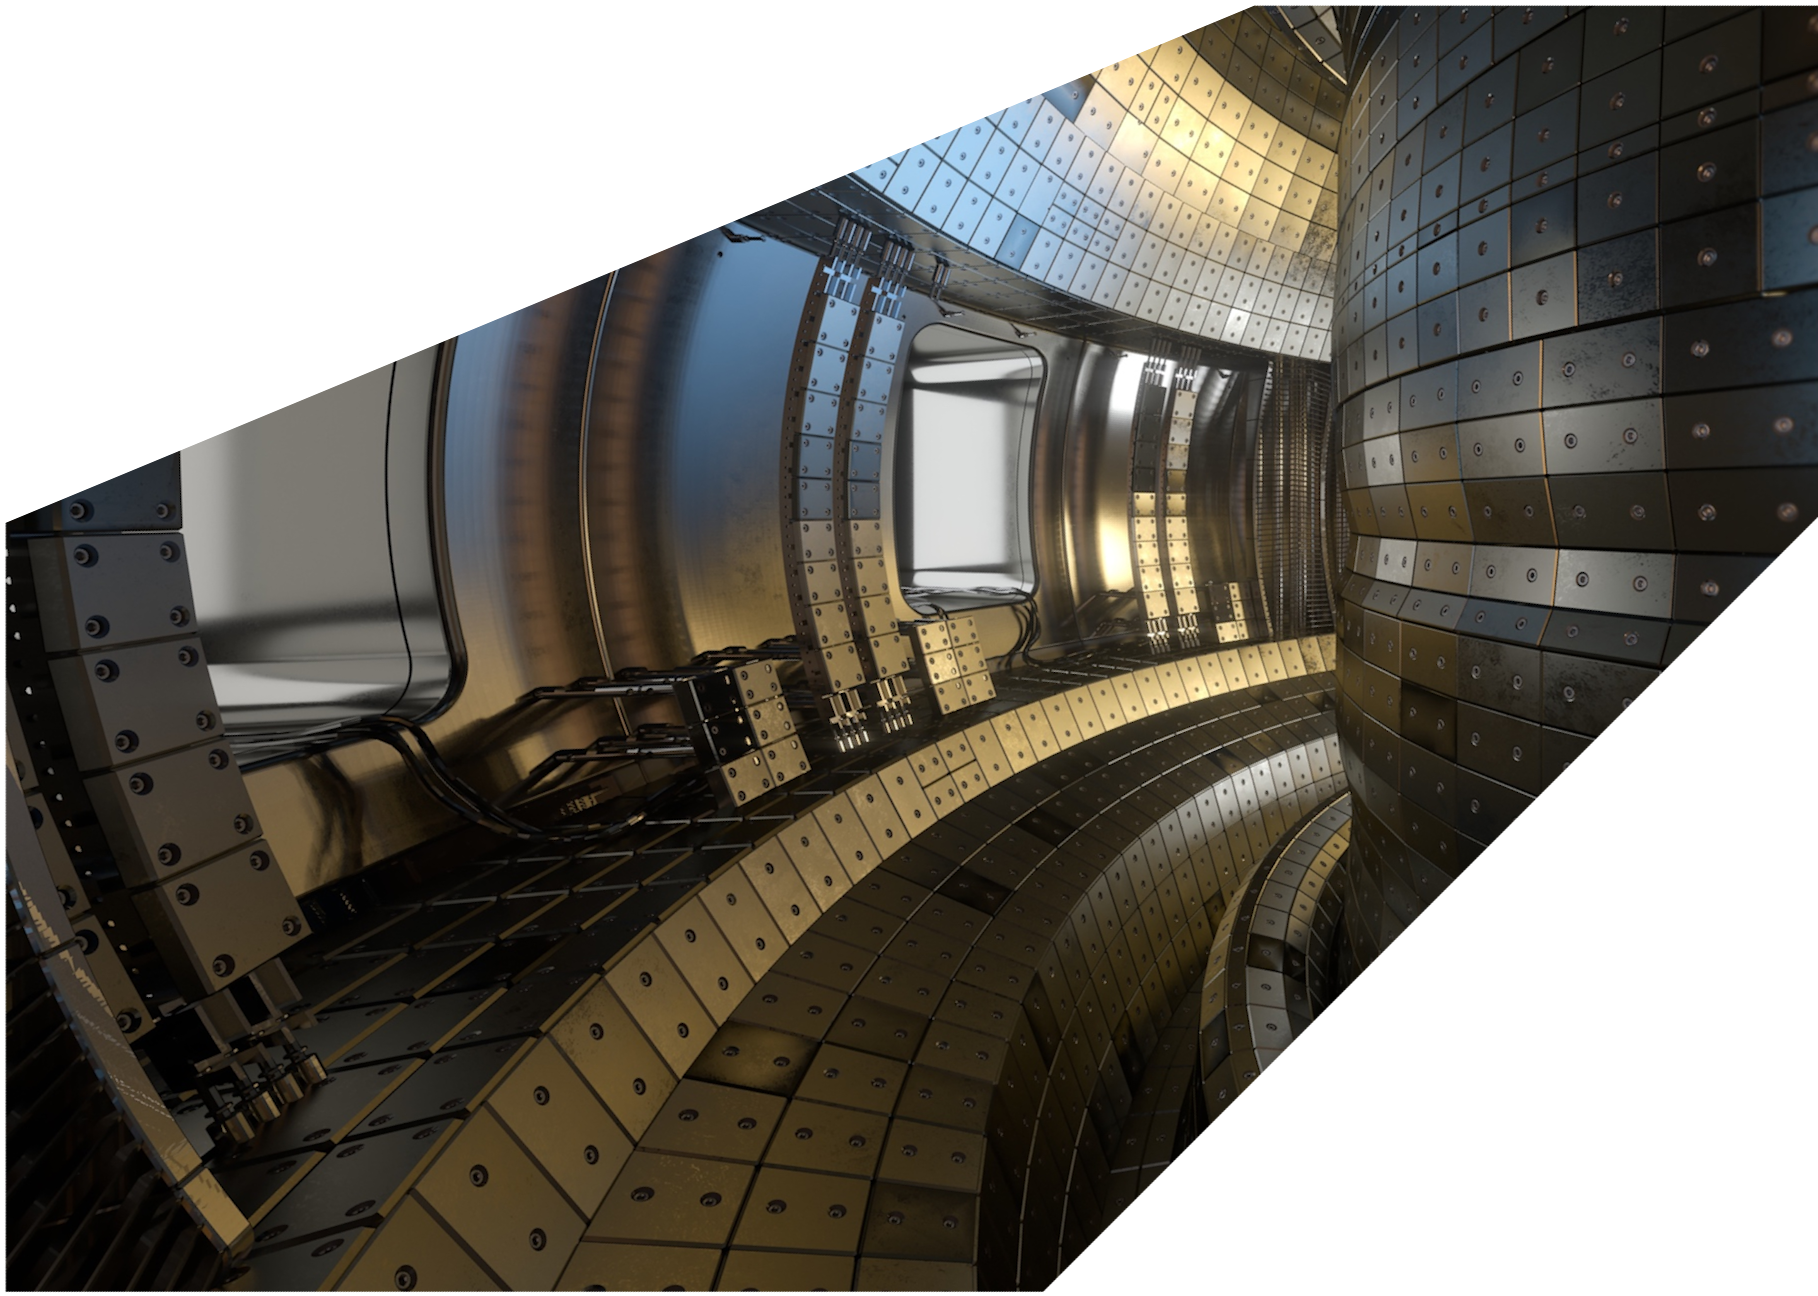
\includegraphics[width=0.9\textwidth]{../corpics/tokintcrop}}%<==omit
\end{titlepage}%<==omit

%\hspace{-30mm}\begin{table}[h]
\sffamily
\begin{center}
\textbf{\textsf{UKAEA REFERENCE AND APPROVAL SHEET}}
\begin{tabular}{||p{5.7cm}|p{4.7cm}|p{5.0cm}||}
\hline
\hline
& Client Reference: &  \\
\hline
& UKAEA Reference: & \culhamshorttitle \\
& & \\
\hline
& Issue: & \culhamissueno \\
\hline
& Date: & \culhamdateb \\
\hline
\multicolumn{3}{||l||}{} \\
\multicolumn{3}{||l||}{Project Name: ExCALIBUR Fusion Modelling System} \\
\multicolumn{3}{||l||}{} \\
\hline
\end{tabular}
\begin{tabular}{||p{3.3cm}|p{4.6cm}|p{3.5cm}|p{3.6cm}||}
\hline
& Name and Department & Signature & Date \\
\hline
Prepared By: & \culhamauthora & N/A & \culhamdate \\
& \culhamauthor & N/A & \culhamdate \\
%& \culhamauthorb  & N/A & \culhamdate \\
%& \culhamauthorc  & N/A & \culhamdate \\
& & & \\
& BD & & \\
\hline
Reviewed By: & \culhamcontactname & 
\includegraphics[width=3.0cm]{../corpics/blanksign}& \culhamdatea \\
& & & \\
& Advanced Computing Dept. Manager & & \\
\hline
%Approved By: & \culhamboardname  & \includegraphics[width=3.0cm]{../corpics/mobsign} & \culhamdateb \\
%& & & \\
%& MSSC & &\\
%\hline
\hline
\end{tabular}
\end{center}
\end{table}


\clearpage
\section{Call Header}
\paragraph*{Call Title}
FM-WP4 Code structure and coordination \ Activity 3.2 - Investigate DSL and code generation techniques (Project \nep\ )
\paragraph*{Value}
12.0pm
\paragraph*{Grant Funds for the period}
100\,\% FEC
\section{Aligns to work package [ FM-WP4 Code structure and coordination ]}
%The  successful bidder will work closely with other community members 
%(especially UKAEA and the successful bidder to Grant Call~T/NA083/20) to produce
%a roadmap to reach the long-term goals of the project. The bidder 
%should indicate how they intend to help drive co-design of all the constituent 
%elements of \nep \   in support of the Fusion Modelling System use case goals 
%and also the \exc \   overarching pillars.

This task will focus upon the suitability of a) available libraries and 
b) numerical algorithms (or possibly the development of new algorithms and/or 
libraries) for the project with a particular focus upon methods for modelling 
anisotropic heat transport. %in the tokamak plasma edge in close proximity to a 
%complex, 3-D first wall.
Summarising the requirements from the Fusion Modelling System Science Plan, of 
particular note for this task is that:

%\item This workpackage will focus upon the suitability of available numerical 
%algorithms (or the development of new algorithms)
%for Exascale targeted plasma modelling, especially anisotropic
%heat transport. As stated in the Fusion Modelling System
%Science Plan, elements of this work package together with FM-WP4 will also
%surround the ``coupling technology'' that will be required to connect the 
%edge/pedestal region of the plasma (addressed
%by FM-WP2) and the neutral gas/impurity model (FM-WP3).
%An agile approach will be adopted around the legacy codes that
%might be necessary for helping to develop a roadmap for the FM-WP1 referent models.
\begin{itemize}
\item  ``\ldots there are a large range of effects in the 
tokamak plasma edge that prevent the plasma from isotropising to a Maxwellian 
distribution \ldots the strong 
imposed and directed magnetic field leads to anisotropy since charged particles 
move rapidly in tight, spiral orbits (gyro-orbits) along the closed field lines 
and only slowly normal to the field", and


\item the ideal numerical algorithms for forming the Exascale edge plasma codes of 
the future will have preferably at least the following properties:
\begin{itemize}
\item[{\bf P1}] Accurate solution of hyperbolic problems.
\item[{\bf P2}] Ability to deliver efficient and accurate solutions of corresponding 
elliptic problems.
\item[{\bf P3}] Accurate modelling of highly anisotropic dynamics. 
\item[{\bf P4}] Accurate representation of first wall geometry (face normals to
within~$0.1^{0}$), and correspondingly of complex magnetic field geometries.
\item[{\bf P5}] Accurate representation of velocity (phase) space.
\item[{\bf P6}] Preservation of conservation properties of the underlying equations.
\item[{\bf P7}] Scalability to likely Exascale architectures:

\begin{itemize}
\item[a)] interaction between models of different dimensionality,
\item[b)] interaction between particle and fluid models,
\item[c)] dynamic construction of surrogates.
\end{itemize}

\item[{\bf P8}] Performance portability to allow rapid deployment upon emerging hardware.
\end{itemize}

\item It is unlikely that any algorithm will have all of the above; part of the exercise
will therefore be to rank the importance of these properties.

%It is difficult at this state to rank the importance of these properties, or to 
%identify the cost associated with
%achieving each in a timely fashion -- a clearer understanding of immediate 
%needs and achievable SMART deliverables will
%emerge as the project matures via extensive community engagement and team 
%building across the UK partners -- this
%exercise will start in Feb 2020 via an open workshop. 

\item It should also be stressed that 
the choice of geometrical representation and numerical 
scheme will have a profound impact upon
almost all areas of the project.

%Options will be identified by means of 
%literature and code surveys and consultation
%with UKRI and industry experts. Research will be commissioned where necessary 
%to eliminate unsuitable choices as early
%as possible. Relatively small development tasks will initially be undertaken to 
%test remaining candidate methods for
%accuracy, stability and HPC scalability potential. \ This task, along with 
%FM-WP4 will have a prioritised start to
%provide initial inputs into FM-WP2 and FM-WP3 developments and work to be 
%defrayed in year 2. Tasks FM-WP1-3 will
%incorporate numerical, finite element and other plasma physics libraries of 
%suitable quality and exascale
%applicability.

\item Options have been tentatively 
identified for initial investigation as
follows:
\begin{enumerate}
\item Spectral/hp element methods
used with Galerkin and/or Discontinuous Galerkin schemes
to meet {\bf P1},{\bf P3} and possibly {\bf P5} above.
\item Nekmesh to meet {\bf P4} above.
\end{enumerate}

\item A critical ``feature" of the fluid referent model prioritised for implementation is
\begin{enumerate}
\item 2-D model of anisotropic heat transport.
\end{enumerate}
\end{itemize}

Elements of work package FM-WP1 together with work managed though FM-WP4 will 
inevitably surround the ``coupling technology" that will be required to 
connect the edge/pedestal region of the plasma (addressed by work managed under 
FM-WP2) and the neutral gas/impurity model (via FM-WP3) -- see Science Plan~\cite{sciplan}. 
Any libraries or algorithms selected must therefore be suitable for the 
Exascale targeted close coupling of models (potentially including both fluid 
and particle-based approaches) that will be essential to deliver a performant 
and actionable infrastructure in the long term.


\section{Objectives}
\nep \  will require the numerical instantiation of systems of equations to deliver
a solution that efficiently and accurately captures
key aspects of the collective physical processes expected to 
operate in the tokamak edge. The allowable systems will treat a range of 
interacting charged and neutral particle species as phase fluids, that is to 
say that functional dependence in velocity space is allowed as well as the more 
usual dependence on space and time. However, only at most two velocity space 
variables should be employed, typically the third will have been removed by 
averaging over the gyro-orbit. Averaging over velocity space 
dependencies to provide fluid-type models only dependent on spatio-temporal variables will be needed.
Plasma species will not only feel the electromagnetic 
field, but may modify its behaviour, which effect must be accounted for. (It 
should be borne in mind that other task packages will address treatment of 
charged and neutral species using discrete particle models and hydrodynamical approaches
involving classical Newtonian fluids, cf.\ Navier-Stokes Equations).

The collective physical processes (regimes) important 
for tokamak edge physics should be determined based on the length scales and timescales observed 
experimentally or derivable from estimates of the number density, temperature 
and magnetic field in the edge, as discussed above for attached L-mode plasmas, and separately
determined in other configurations. It is expected that 
relevant processes for each species separately will be selected on the basis of 
a small number of key parameters, of which obviously the first is number 
of particles of each species in the Debye sphere that should be large to ensure that a plasma 
treatment is appropriate. The second will be magnetisation parameter~$\delta_s=\rho_{ts}/L$ of a 
representative species particle, others will include the normalised collision 
frequency~$\nu^{*}=L/\lambda_{smfp}$, the drift-ratio, the
width of the SOL normalised to~$L$ and the plasma~$\beta$.
Different models will be appropriate according 
to the relative sizes of these latter key parameters, and the magnetic 
geometry, that is to say whether field lines are (i) straight (slab 
geometry), (ii) twisted, (iii) toroidal, (iv) twisted and toroidal. Note the 
term ``model" includes not only say special collision operators appropriate 
to interaction between different species including neutral species, but also 
the boundary conditions appropriate to the particular physical case, or for the 
latter it may be acceptable to describe how the representation changes to 
particle and/or hydrodynamic fluid on a bounding surface or over an overlap 
volume. In all cases, the limitations of each model need to be clearly stated, including a 
discussion of the ease of its numerical implementation at the Exascale.

The identification of key edge physical processes and regimes will prioritise 
the theoretical developments needed to produce models capable of treating them 
efficiently at the Exascale. Ideally it should be possible to transition smoothly 
from one model to another as key parameters vary, both as time varies and as a 
function of position. It is expected that the widely differing timescales for 
electron and ion species dynamics will present a particular challenge, and 
interaction is expected with other tasks for designing software for multiscale 
applications and researching surrogate models. Theorists are also expected to 
collaborate with numerical experts not only in respect of ease of implementation, 
but also to produce algorithms for estimating likely errors, both within a 
single species model and in its interactions with other species models 
including discrete particle and hydrodynamical fluid, in order to guide refinements 
to the equations of the system describing the given regime.

\section{Anticipated outputs and results}
\begin{enumerate}
\item Document describing documentation standards for the project,
with a section contrasting choices made different from UK Met Office
\item Document describing testing framework for the project,
with a section contrasting choices made different from UK Met Office
\item Design of repository structure (repository or subdirectories of repository)
to contain project files, initially populated with above documents
\item Tools to assist in the production of consistent documentation
and ease production of test cases. These may be multi-provenance, ie.\
selected from existing
software, represent modification of such tools or be specially written
\item  Design of repository structure to contain information
and other input and output data needed for testing software developed under \nep ,
especially \papp s, and including multi-provenance software for
pre- and post-processing, initially populated with results of at least one \papp .
\item Design of repository structure to contain
software developed under \nep\ especially \papp s, with capability to
produce executables, initially populated with at least one \papp .
\item Training material for documentation standards and the testing framework
\end{enumerate}

(Access to UK Met Office repositories may be arranged through \exc if needed.)


\begin{table}[h]
\textbf{\textsf{GLOSSARY:}}
\begin{center}
\begin{tabular}{|p{4.0cm}|p{12.0cm}|}
\hline
\textbf{\textsf{Term or Acronym}}
& \textbf{\textsf{Definition}} \\
C++ & Programming language, see \url{https://isocpp.org/} \\
DPC++ & Data Parallel C++, Intel compiler for C++ with SYCL extension \\
DSL & Domain Specific Language, programming language developed for a specific area of resrearch and development \\
Object Fortran & Programming language, more precisely Fortran~95 or later exploiting object-oriented features of the language, see \url{https://wg5-fortran.org/f2008.html} \\
Python & Programming language, see \url{https://python.org/} \\
SYCL & C++ library  for portable high performance computing, see \url{https://www.khronos.org/sycl/} \\
Kokkos & C++ library for portable high performance computing \url{https://cfwebprod.sandia.gov/cfdocs/CompResearch/docs/Kokkos-Multi-CoE.pdf} \\
OpenMP & Software for parallel programming \\
SRO & Senior Responsible Owner role in UK  government project delivery \\
Julia & Programming language, see \url{https://julialang.org/} \\
UKRI & United Kingdom Research and Innovation, a non-departmental public body encompassing the research councils and Innovate UK \\
VVUQ & Verification, Validation and Uncertainty Quantification \\
\hline
\end{tabular}
\end{center}
\end{table}

%\bibliographystyle{unsrt}
%\bibliography{../bib/new,../bib/waynes,../bib/misc,../bib/warv,../bib/neuts,../bib/reac,../bib/exc,../bib/active,../bib/dg1srt}

\end{document}
